%\documentclass[preprint,12pt]{elsarticle}

%% Use the option review to obtain double line spacing
%% \documentclass[preprint,review,12pt]{elsarticle}

%% Use the options 1p,twocolumn; 3p; 3p,twocolumn; 5p; or 5p,twocolumn
%% for a journal layout:
%% \documentclass[final,1p,times]{elsarticle}
%% \documentclass[final,1p,times,twocolumn]{elsarticle}
%% \documentclass[final,3p,times]{elsarticle}
\documentclass[final,3p,times,twocolumn]{elsarticle}
%% \documentclass[final,5p,times]{elsarticle}
%% \documentclass[final,5p,times,twocolumn]{elsarticle}

\usepackage{amsmath}
%\usepackage{amssymb}
%\usepackage{amsthm}
%\usepackage{makeidx}
\usepackage{graphicx}
%\usepackage[pdftex]{graphicx}
\usepackage{subfig}

%% natbib.sty is loaded by default. However, natbib options can be
%% provided with \biboptions{...} command. Following options are
%% valid:
%%
%%   round  -  round parentheses are used (default)
%%   square -  square brackets are used   [option]
%%   curly  -  curly braces are used      {option}
%%   angle  -  angle brackets are used    <option>
%%   semicolon  -  multiple citations separated by semi-colon
%%   colon  - same as semicolon, an earlier confusion
%%   comma  -  separated by comma
%%   numbers-  selects numerical citations
%%   super  -  numerical citations as superscripts
%%   sort   -  sorts multiple citations according to order in ref. list
%%   sort&compress   -  like sort, but also compresses numerical citations
%%   compress - compresses without sorting
%%
%% \biboptions{comma,round}
% \biboptions{}


\def\wrt{w.\,r.\,t.\ }
\def\eg{e.\,g.\ }
\def\ie{i.\,e.\ }
\def\Dash{\nobreak\,---\penalty-500\,}

%%% Comments
\usepackage{color}
\newcommand{\TG}[1]{{\color{blue}\textbf{TG: #1}}}
\newcommand{\CD}[1]{{\color{green}\textbf{CD: #1}}}
\newcommand{\IP}[1]{{\color{cyan}\textbf{IP: #1}}}
\newcommand{\TODO}[1]{{\color{red}\textbf{TODO: #1}}}
%%%

\renewcommand{\Vec}[1]{\boldsymbol{#1}}
\newcommand{\Mat}[1]{\boldsymbol{#1}}


\journal{Medical Image Analysis}

\begin{document}

\begin{frontmatter}

%% Title, authors and addresses

%% use the tnoteref command within \title for footnotes;
%% use the tnotetext command for the associated footnote;
%% use the fnref command within \author or \address for footnotes;
%% use the fntext command for the associated footnote;
%% use the corref command within \author for corresponding author footnotes;
%% use the cortext command for the associated footnote;
%% use the ead command for the email address,
%% and the form \ead[url] for the home page:
%%
%% \title{Title\tnoteref{label1}}
%% \tnotetext[label1]{}
%% \author{Name\corref{cor1}\fnref{label2}}
%% \ead{email address}
%% \ead[url]{home page}
%% \fntext[label2]{}
%% \cortext[cor1]{}
%% \address{Address\fnref{label3}}
%% \fntext[label3]{}

\title{TODO: Title} % TODO

%% use optional labels to link authors explicitly to addresses:
%% \author[label1,label2]{<author name>}
%% \address[label1]{<address>}
%% \address[label2]{<address>}

\author{}

\address{}

\begin{abstract}
%% Text of abstract
TODO % TODO
\end{abstract}

\begin{keyword}
deformable liver model \sep Glisson's capsule \sep vascularization \sep real-time soft tissue modeling

%% MSC codes here, in the form: \MSC code \sep code
%% or \MSC[2008] code \sep code (2000 is the default)

\end{keyword}

\end{frontmatter}

% ---  Main text  ---

\TG{mostly just copy of MICCAI paper}

\section{Introduction} %{{{

According to the statistics, nearly 100,000 European citizens die of cirrhosis or liver cancer each year. 
Although new methods such as radio-frequency- and cryo-ablation known in the interventional radiology 
seem to be promising, surgery remains the option that offers the foremost success rate against these pathologies. 
Nevertheless, surgery is not always performed due to several limitations, in particular the determination 
of accurate eligibility criteria for the patient. 
In this context, the pre-operational planning becomes a crucial task having a significant impact on the treatment. 

Computer-aided physics-based medical simulation has proven to be an extremely useful technique in the area of medical training. 
Nevertheless, whereas generic models are usually required in training simulators, accurate patient-specific modelling
becomes necessary as soon as computer simulation is to be employed in the pre-operative planning. At the same time, 
interactivity of such models remains an important aspect, requiring real-time simulation which is often difficult to 
achieve given the complexity of soft tissues. 

When simulating the behavior of human liver, the task of real-time accurate modeling is challenging, mainly because of the complex structure 
of this organ composed of three main constituents: \emph{parenchyma}, \emph{vascular networks} and \emph{Glisson's capsule}.
The parenchyma has certainly been the most studied component of the liver; actually researchers agree on hyperelastic 
properties of the tissue, for which the mechanical parameters have been reported for example in~\cite{Kerdok2006,Gao2009}. 
Moreover, several methods have been proposed to model the hyperelastic behaviour at real-time rates, such as multiplicative Jacobian decomposition
introduced in~\cite{Marchesseau2010}.

The mechanical importance of the vascular structures in liver is studied in~\cite{Peterlik2012}. It shows that the 
influence of vessels on the mechanical behaviour of the organ is significant, mainly if large deformations occur. 
Since a detailed modeling of the vessels would be extremely costly (mainly because of the small thickness of the vessel wall, 
the authors propose a composite model allowing for real-time simulation of entire liver with vascularization.

Rather a small number of studies have been conducted dealing with the third liver constituent, the  Glisson's capsule.
Quantitative results of experiments on a porcine liver have been published in~\cite{Umale2011}; the measurements indicate that although being very 
thin (10--20$\mu m$), the capsule shows to be stiff in tensile tests: the Young's modulus of the capsule reported to be $8.22\pm3.42$\,MPa 
exceeds the values for the parenchyma by three orders of magnitude.
This suggests that the mechanical influence of the membrane on the liver behaviour is not negligible.

In~\cite{Hollenstein2006}, a local influence of the capsule has been measured using a special aspiration device. The study was then repeated 
in vivo on human patients during the operation, confirming the mechanical importance of the membrane~\cite{Ahn2010,Nava2008}.
To our best knowledge, no attempt has been made to demonstrate the role of the Glisson's capsule on the global behaviour of 
the liver, mainly if the organ undergoes large deformations which is often the case during the surgery.

The main contribution of the paper is twofold: first, we present a real-time model of the liver, including
the parenchyma, vascularization and Glisson's capsule. The model is based on three different finite element representations for each constituent,
linked together via mechanical coupling. We show that the model mimics the \emph{local} experiments described in~\cite{Hollenstein2006}.
 
Second, we use the complete model of the liver to demonstrate the \emph{global} influence of the Glisson's
capsule via simulation: using a specific model of a porcine liver built from CT contrast-enhanced data, we show that there is a significant 
difference in the response of the model with and without the capsule in the case when the liver undergoes large deformations. 

The paper is organized as follows: first we describe the proposed vascularized
liver model with capsule. Second, we validate our model in context of local deformations by reproducing the aspiration test 
described in~\cite{Hollenstein2006}. Finally, we demonstrate that in spite of its small thickness, the Glisson's 
capsule has a global influence on the liver undergoing large deformations. 

%}}}


\section{Model} %{{{

In this section we describe the construction of a composite model
based on three components: tetrahedral FE model of the 
parenchyma, Tymoshenko-beam model for the vascular structures and finally 
triangular membrane elements used for the capsule.

\subsection{Parenchyma} %{{{

It is known that the parenchyma exhibits non-linear viscoelastic behaviour
\cite{Marchesseau2010,Gao2009}.
However, as we are mainly interested in the static equilibrium, we do not model the time-dependent
phenomena related to viscosity.

%However, we employ simpler corotational model as we are not so much
%interested in time-dependent behaviour but rather in static equilibrium
%under certain conditions.
%We also rely on the vascularized model of the parenchyma proposed by
%Peterl\'{i}k et al. \cite{Peterlik2012}.

The parenchyma is modeled using corotational finite elements~\cite{Felippa2005}.
Although it relies on linear stress-strain relationship, large displacements including rotations are modelled correctly. 
While in the full non-linear formulation the stiffness matrix relates the forces $\Vec{f}$ and 
displacements $\Vec{u}$ as $\Vec{f} = \Mat{K}(\Vec{u})$, the corotational model 
requires the stiffness matrix $\Mat{K}_0$ of the system to be computed only once before the simulation begins. 
Then, in each step, the motion of each element $e$ is decomposed into rigid rotation $\Mat{R}^e$ and local deformation. 
The rotations are then used to update each local element stiffness matrix as $\Mat{R}\Mat{K}_0\Mat{R}^{\top}$
whereas the deformations are used to compute the linear strain in the local corotational frame.
%The stiffness matrix $\Mat{K}$ can be expressed in terms of the deformation
%$u$ and the force as $\Vec{f} = \Mat{K}(\Vec{u}) \Vec{u}$. 
%Where the
%components of $\Mat{K}$ depend on the orientation of each element in the
%current simulation step.
%the rigid component is  
% The corotational
%formulation allows us to deal with geometrical non-linearities but still
%relies on linear stress-strain relationship. Thus rotations and large
%deformations are modelled correctly. 
%In the corotational formulation the deformation
%of each element is expressed in the local frame of reference. 
There are several ways of computing the corotational frame for elements; we rely on
the geometrical method proposed in \cite{Nesme2005}.
% NOTE: This description of corotational method is very simplified and could be extended.

%}}}

\subsection{Vascularization} %{{{

As a first step towards a mechanical model of vessels, a continuous
representation of vascular structures is constructed. Using segmeted data
of a vessel tere, points along centerlines of each vessel branch are
selected. This task can be performed either manually or automatically, \eg
with VMTK\footnote{www.vmtk.org}. Each branch can be represented as a
series of cubic B\'{e}zier curves fitted to the centerline points: the
series begins in a starting point of the branch and ends either in another
branching point or in the endpoint of the branch.

A set of interpolated points is constructed using the B\'{e}zier curves;
positions of the interpolated points can be chosen arbitrarily along each
branch dividing it ionto intervals with a constant or varying length. For
each interpolated point we calculate its orientation given by the tangent
and normal of the B\'{e}zier curve in that point.

The interpolated points are used as nodes of serially linked beam elements,
in a similar way as proposed by Duriez et al. \cite{Duriez2006} for
simulating catheters and guidewires. This model shares some similarities
with the corotational model described above, and in particular allows for
geometrically non-linear deformations. We introduce some modifications to
the model to take into account particular nature of vessels, in particualr
through specific cross section profiles and moments of inertia (see
\cite{Przemieniecki1985} for details). The static formulation for the
deformation of a beam is described by a system similar to the one used for
the parenchyme, with the difference that each node is described with six
degrees of freedom, three of which correspond to the spatial position, and
three to the angular position of the node in a global reference frame
\TODO{figure?}.


% TODO: presunout do sekce composite model
%The beam-based model of vessels is mechanically coupled to the parenchyma as described in~\cite{Peterlik2012}. 
%The coupling assumes that there is no relative motion between the vessels and the surrounding parenchyma. 
%%The proposed model assumes no relative
%%motion of vessels to the parenchyma. Segmented vascular network is
%%discretized into the set of linear elements that are then projected into
%%the tetrahedral mesh of the parenchyma. 
%During the simulation, the nodes of linked beams are first displaced and rotated according to the actual motion of associated tetrahedra. 
%As the deformation of beams results in mechanical response represented by forces and torques, these are propagated back to 
%the tetrahedral FE model. 

%%a displacement of tetrahedral nodes are mapped  forces and torques resulting from the deformations of vessels by parenchyma are
%%computed and propagated back onto the tetrahedral mesh.

%}}}

\subsection{Glisson's Capsule} %{{{
\label{ss:capsuleModel}
The thickness of the Glisson's capsule is relatively small: the values in range of 10-20
$\mu$m have been reported in~\cite{Umale2011}.
It is not possible to model such thin structure with classical tetrahedral
elements, if the real-time aspect of the simulation is to be preserved.
Furthermore, modeling both the tissue and the capsule would require an extremely 
dense mesh to avoid numerical instabilities and thus would significantly
violate the speed requirements imposed for medical simulators.
Instead, modeling the capsule with two-dimensional elements that abstract from the
thickness in the third dimension seems
to be a natural choice. In the elasticity theory, this functionality is usually provided by membrane and shell elements.
Based on the observation of its behaviour, we also
assume negligible bending forces and propose a model based on membrane
elements. 
To maintain simplicity of the composite model we choose simple triangular
elements with constant strain (CST).

The computation of elastic stiffness matrix follows the common derivation
%
\begin{eqnarray}
  \Mat{K}^m & = & \int_V \Mat{B}^T \Mat{E} \Mat{B} dV     \label{mem1} \\
            & = & h \int_A \Mat{B}^T \Mat{E} \Mat{B} dA   \label{mem2} \\
            & = & h A \Mat{B}^T \Mat{E} \Mat{B}           \label{mem3}
\end{eqnarray}
%
where $\Mat{B}$ is the strain-displacement matrix, $\Mat{E}$ the material
matrix, $h$ is the thickness and $A$ area of the element. In the previous
\eqref{mem2} follows from the fact that we assume constant thickness of the
element and \eqref{mem3} follows from the fact that the strain-displacement
matrix is constant in our case. The strain-displacement matrix for the CST
element can be expressed as:
%
\begin{equation}
  \Mat{B} = \frac{1}{2A} \begin{bmatrix}
    y_{23} & 0      & y_{31} & 0      & y_{12} & 0 \\
         0 & x_{32} & 0      & x_{13} & 0      & x_{21} \\
    x_{32} & y_{23} & x_{13} & y_{31} & x_{21} & y_{12}
  \end{bmatrix}
\end{equation}
%
The values $x_{ij} = x_i - x_j$ and $y_{ij} = y_i - y_j$ are computed from
the $x$ or $y$ coordinates of the nodes $i,j$ of the triangular element.
The reader can refer to the respective literature for more thorough
description~\cite{Felippa2003}.

We use linear elastic material and employ the corotational formulation
for the CST elements.

%}}}


\subsection{Coupling Between Vessels and Parenchyma} %{{{

We propose a mapping betwen the mesh nodes of the vessels and parenchyma to
create the vascularized model. Since no relative motion between the vessels
and parenchyma is observed in reality, the mapping betweeen the two can be
modelled as a constraint. In each step of the simulation, the actual
displacements of the parenchyma mesh nodes are mapped to the vessel nodes
and reciprocally, the force contribution due to the deformation of the
vessel is propagated to the parenchyma. The mapping of the forces is based
on a principle of virtual work. Using the corotational model, the
parenchyma is discretized by a mesh composed of a linear $P_1$ tetrahedral
elements given by four nodes with three degrees of freedom. The vessel is
modeled with beam elements where each beam is given by two end points each
having 6 degreees of freedom (positions and rotations). We focus on mapping
betwen an arbitrary beam node $b$ and tetrahedron $T$.

Let us denote $\Vec{p}$ the initial position and $\Mat{R}$ initial rotation
of the beam node $b$. Before the simulation starts, we select the
tetrahedron $T = \{\Vec{t}_A, \Vec{t}_B, \Vec{t}_C, \Vec{t}_D \}$ which is
closest to the beam node $b$. Then, the barycentric coordinates
$\Vec{\beta}_T = \{\beta_A, \beta_B, \beta_C\}$ of the position $\Vec{p}$
are computed \wrt the tetrahedron $T$ and stored. Similarly, the initial
rotation $\Mat{R}$ is transformed to a a matrix $\Mat{O}_T$ which defines
the orientation of the point $B$ \wrt the local basis $\Mat{L}$ defined by
the edges of the tetrahedron, \ie $\Mat{O}_T = \Mat{L}^{-1} \Mat{R}$.
According to the initial assumption (no relative motion between parenchyma
and vessel), both the barycentric coordinates $\Vec{\beta}_T$ and
$\Mat{O}_T$ are constant during the simulation. Let's suppose that in  the
actual step, the tetrahedron is rotated and deformed as shown in
\TODO{figure}. Denoting the nodal positions of the deformed tetrahedron $T'
= \{\Vec{t}'_A, \Vec{t}'_B, \Vec{t}'_C, \Vec{t}'_D\}$, new actual position
$\Vec{p}'$  of the beam node is computed using the barycentric coordinates
$\Vec{\beta}_T$ as
%
\begin{equation}
  \Vec{p}' = \Vec{t}'_A \beta_A + \Vec{t}'_B \beta_B + \Vec{t}'_C \beta_C +
  \Vec{t}'_D (1 - \beta_A - \beta_B - \beta_C).
\end{equation}
%
The updated orientation $\Mat{R}'$ of the beam node is computed using the
basis $\Mat{L}'$ given by the actual displacement of the tetrahedron nodes
and precomputed orientation $\Mat{O}_T$. First, $\Mat{\tilde{R}}' =
\Mat{L}' \Mat{O}_T$ is computed. However, since besides the rotation ad
deformation of the tetrahedron must be taken into account the matrix
$\Mat{\tilde{R}}'$ is not necessarily orthogonal. Therefore, the updated
orientation $\Mat{R}'$ is calculated as orthogonal component of polar
decomposition of $\Mat{\tilde{R}}'$. As the positional mapping is applied
in each step of the simulation, the positions of the beams are
kinematically linked to the positions of tetrahedra.

After the updated position is mapped from the tetrahedron to the beam point,
the forces acting in the beam point must be mapped onto the vertices of the
associated tetrahedron. For the beam point, we have linear forces $\Vec{f}
= \{ f_x , f_y , f_z \}$
as well as torques $\Vec{\tau} = \{ \tau_x, \tau_y, \tau_z \}$, whereas for the tetrahedron, there are only
linear nodal forces $\Mat{F} = \{ \Vec{f}_A , \Vec{f}_B , \Vec{f}_C ,
\Vec{f}_D \}$ . The force contribution to each node
given by linear forces f is computed using the barycentric coordinates, required
by the positional mapping. The torques are transformed to linear forces acting in
the tetrahedron nodes using the equation $\Vec{\tau} = \Vec{r} \times
\Vec{f}$ where $\Vec{r}$ is vector connecting
the beam and tetrahedron nodes. Putting it together, the force in tetrahedron
node $I \in \{A, B, C, D\}$ is computed as $\Vec{F}_I = \beta_I \Vec{f} −
(\Vec{t}'_I − \Vec{p}') \times \tau$.


%}}}

\subsection{Coupling Between Capsule and Parenchyma} %{{{
The literature reports high cohesion between capsule and parenchyma
\TODO{need refs}.
Based on this property we assume there is no relative motion of the capsule \wrt the parenchyma.
Although an arbitrary surface mesh could be used to model the capsule, we exploit 
the fact that the parenchyma is modeled by tetrahedral elements having
triangular faces. Thus, as the boundary of the volumetric mesh is already
triangulated, we simply employ the triangles on the mesh surface to model the capsule.

Using directly the boundary of the tetrahedral mesh does not only solve the
problem of building the surface mesh, but has one more advantage: the nodes
of the triangular mesh coincide with the nodes of the tetrahedral mesh, so no projection of one mesh onto the other is needed.
Moreover, the stiffness matrices for capsule and parenchyma are then easily assembled
together.
% and solved as one system.
%
%\CD{The following may appear as "trivial"... maybe we can remove this part at the end if we need space} 
%Without the loss of generality we can assume the tetrahedron consists of
%nodes $p_1, p_2, p_3$ and $p_4$ and the boundary triangle has nodes $p_1, p_2$
%and $p_3$. We can reorder the degrees of freedom so that the stiffness
%matrix $\Mat{K}^t$ for the tetrahedron can be written as:
%%
%\begin{equation}
%  \Mat{K}^t = \left[\begin{array}{c|c}
%      \Mat{K}^t_{1-3,1-3} & \Mat{K}^t_{1-3,4} \\
%      \hline
%      \Mat{K}^t_{4,1-3} & \Mat{K}^t_{4,4} \\
%  \end{array}\right]
%\end{equation}
%%
%Then the assembled stiffness matrix for the element is:
%%
%\begin{equation}
%  \Mat{K} = \left[\begin{array}{c|c}
%      \Mat{K}^t_{1-3,1-3} & \Mat{K}^t_{1-3,4} \\
%      \hline
%      \Mat{K}^t_{4,1-3} & \Mat{K}^t_{4,4} \\
%  \end{array}\right]
%  +
%  \left[\begin{array}{c|c}
%      \Mat{K}^m & 0 \\
%      \hline
%      0 & 0 \\
%  \end{array}\right]
%\end{equation}
%%
%Where $\Mat{K}^m$ is the stiffness matrix of the triangular membrane.
The resulting system of linear equations is solved by direct solver based on Cholesky decomposition.

%}}}

%}}}


\section{Experiments} %{{{
The model presented in the previous section was implemented in 
SOFA\footnote{www.sofa-framework.org} and a set of
numerical simulations was performed. First, local deformations were compared to the
results reported in literature to validate the method.
Second, to show that in spite of its very small thickness the membrane cannot be
neglected even in the context of global deformations and its overall
stiffness plays an important role, the model of
the complete liver was subjected to global deformations.

In the simulations we used material properties reported in the literature: for the 
Glisson's capsule we used Young's modulus $E_c$=8.22\,MPa and thickness $t_c$=20\,$\mu$m~\cite{Umale2011},
whereas for the vessel wall we applied stiffness $E_v$=0.62\,MPa and thickness $t_v$=200\,$\mu$m~\cite{Peterlik2012}.
Since the values for parenchyma elasticity quite vary (usually between 2\,kPa to 5\,kPa), we perform the simulation 
with $E_p$=3.5\,kPa.

%XXX
%\begin{figure}[t]
%    	\subfigure[]{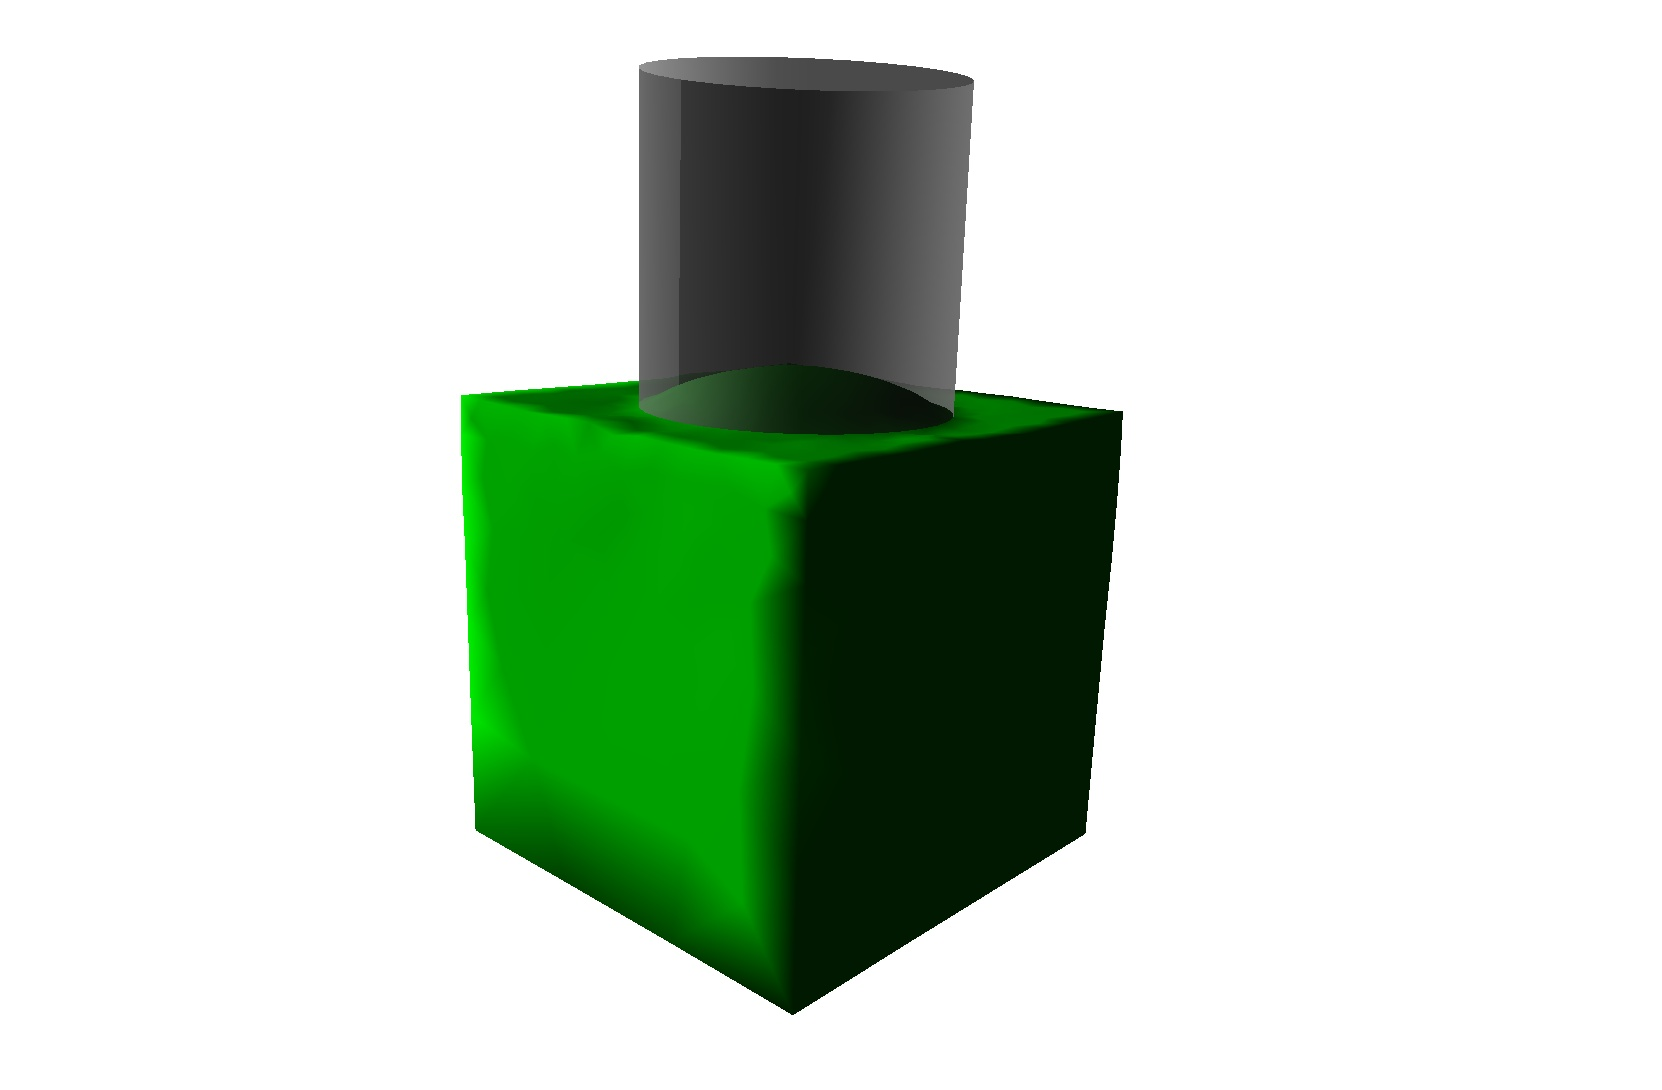
\includegraphics[height=3.5cm]{aspiration.jpg}}
%	\subfigure[]{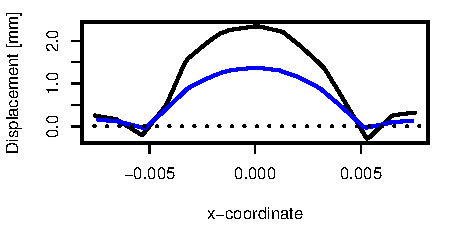
\includegraphics[width=7cm]{aspiration.pdf}}
%  \caption{\label{fig-aspiration}Aspiration test: (a) the SOFA simulation scene, (b) cube displacement profile
%  with the capsule (in blue) and without capsule (in black).}
%\end{figure}

\subsection{Local Deformations} %{{{
During the contact with an instrument such as probe, needle, scalpel and others,
a specific deformations take place in the vicinity of
the instrument. This type of deformation may not necessarily induce the
deformation of the object as a whole and therefore can be considered as
local. Correct material properties are not only important to quantify the
displacement, but also play an important role in capturing the correct area of
the deformation or its profile near the instrument.

A good example of such a local deformation is the aspiration test
where the response of liver exposed locally to a negative pressure is measured.
In~\cite{Hollenstein2006} it is reported that the Glisson's
capsule has a non-negligible influence on the response of the tissue and modeling
only the parenchyma leads to an overestimation of the deformation. 
%We reproduced the test with our model and acquired similar results.
The aspiration device consists of a tube 1\,cm in diameter and allows
to control internal pressure in the tube. The test is performed by
attaching the tube to the tissue and measuring the tissue response. We
set up a simulation in SOFA to reproduce the experiment (see Fig.~\ref{fig-aspiration}a): we meshed a 15$\times$15$\times$15\,mm$^3$ 
cube representing the tissue 
resulting in 2648 tetrahedra. Then we attached a 1\,cm tube 
and applied a pressure of 3\,kPa inside the tube. The interaction between the tube and 
tissue was modelled with friction contact. 

In Fig.~\ref{fig-aspiration}b the profiles of cuts in the middle of the
test cube are presented showing significantly larger deformation in the model without capsule. This is in perfect 
agreement with the results reported in~\cite{Hollenstein2006} and it can be concluded that 
our composite model based on coupling the triangular and tetrahedral elements provides an accurate 
model of parenchyma and capsule.

---

Since the tube is in direct contact with the tissue, uni-lateral constraints with friction were chosen 
to model this interaction properly. We opted for a method based on \emph{non-linear complementarity problem}  (NLCP)
where the non-linearity is introduced due to the friction. The NLCP
allows for solution of the Signorini's problem to avoid any interpenetration between the colliding 
objects (see~\cite{Duriez2006b} for details). Since NLCP requires explicitly the computation of compliance matrix which 
is homogeneous to the inverse of the stiffness matrix, we employed a direct solver based on LDL decomposition to 
solve the system and compute the inverse matrices. 


As the first step, we evaluate the influence of the Glisson's capsule on the mechanical response of the tissue during
the aspiration test. 
In~\cite{Hollenstein2006} it is reported that the influence of the capsule is significant, as modeling 
only the parenchyma without considering the membrane results in overestimation of the deformation by a factor of 2 to 3. 
In order to verify this observation, we performed a simulation using capsule parameters measured experimentally on 
ex-vivo pig liver~\cite{Umale2011}: Young's modulus of the membrane was set to $E_c$=8.22\,MPa and thickness was
$t_c$=20\,$\mu$m. 
Since the values for parenchyma elasticity reported in the literature vary significantly being usually reported between 2\,kPa to 5\,kPa, 
we employed a value $E_p$=3.5\,kPa for the Young's modulus of the parenchyma. 

%\begin{figure}
%  \centering
%  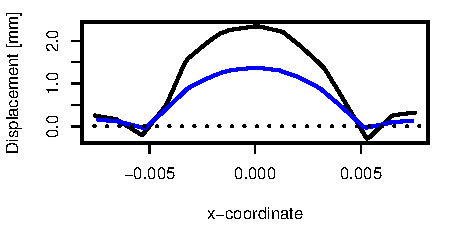
\includegraphics[width=7cm]{aspiration.pdf}
%  \caption{\label{fig-aspiration2} Displacement profile of the cube in the
%  aspiration test with (blue) and without (black) the capsule.}
%\end{figure}
%
%\begin{figure}
%  \centering
%  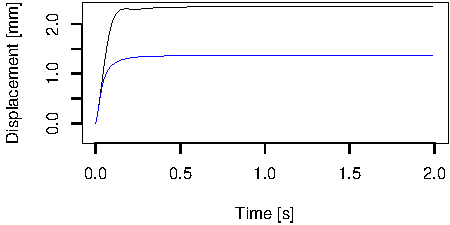
\includegraphics[height=3.5cm]{displacement.pdf}
%  \caption{\label{fig-aspiration3} Evolution of the displacement at the center
%  in time for test with (blue) and without (black) the capsule.}
%\end{figure}

In Fig.~\ref{fig-aspiration2} the profiles of cuts in the middle of the
test cube are presented showing significantly larger deformation in the model without capsule assuming that the same negative pressure was applied 
on the tissue surface inside the tube. Moreover, it can be observed that the deformation without capsule is overestimated by a factor 
close to 2, which is in perfect agreement with the results reported in~\cite{Hollenstein2006}.

In the second step, we employed the simulation to reproduce the displacements values obtained via simulation in~\cite{Hollenstein2006,Nava2008}.
Whereas the simulation in the referenced work was done on a mesh composed of tetrahedral elements for both the parenchyma 
and the capsule, we modeled the capsule using the triangular elements as shown in section~\ref{ss:capsuleModel}.

Since the Young's moduli of neither parenchyma ($E_p$) nor capsule ($E_c$) were specified exactly, we obtained both as follows: first, 
we performed a set of simulations without the capsule for different values of $E_p$: the value that provided a good match 
with reported displacements was $E_p$=30\,kPa. 
Then, we fixed the thickness of the capsule to be $t$=93\,$\mu$m (reported as the average value in the paper) and 
using $E_p$=30\,kPa, we ran the simulation repeatedly using the model with the capsule. In each simulation we 
used different value $E_c$ of the Young's modulus for the capsule in order to minimize the displacement error w.r.t. the 
reported values. The minimal value of error (not exceeding 1\%) was obtained for $E_c$=3\,MPa. This 
value lies in the range of capsule elasticity coefficients reported by experimental measurements.



%}}}

%XXX
%\begin{figure}[t]
%  \centering
%    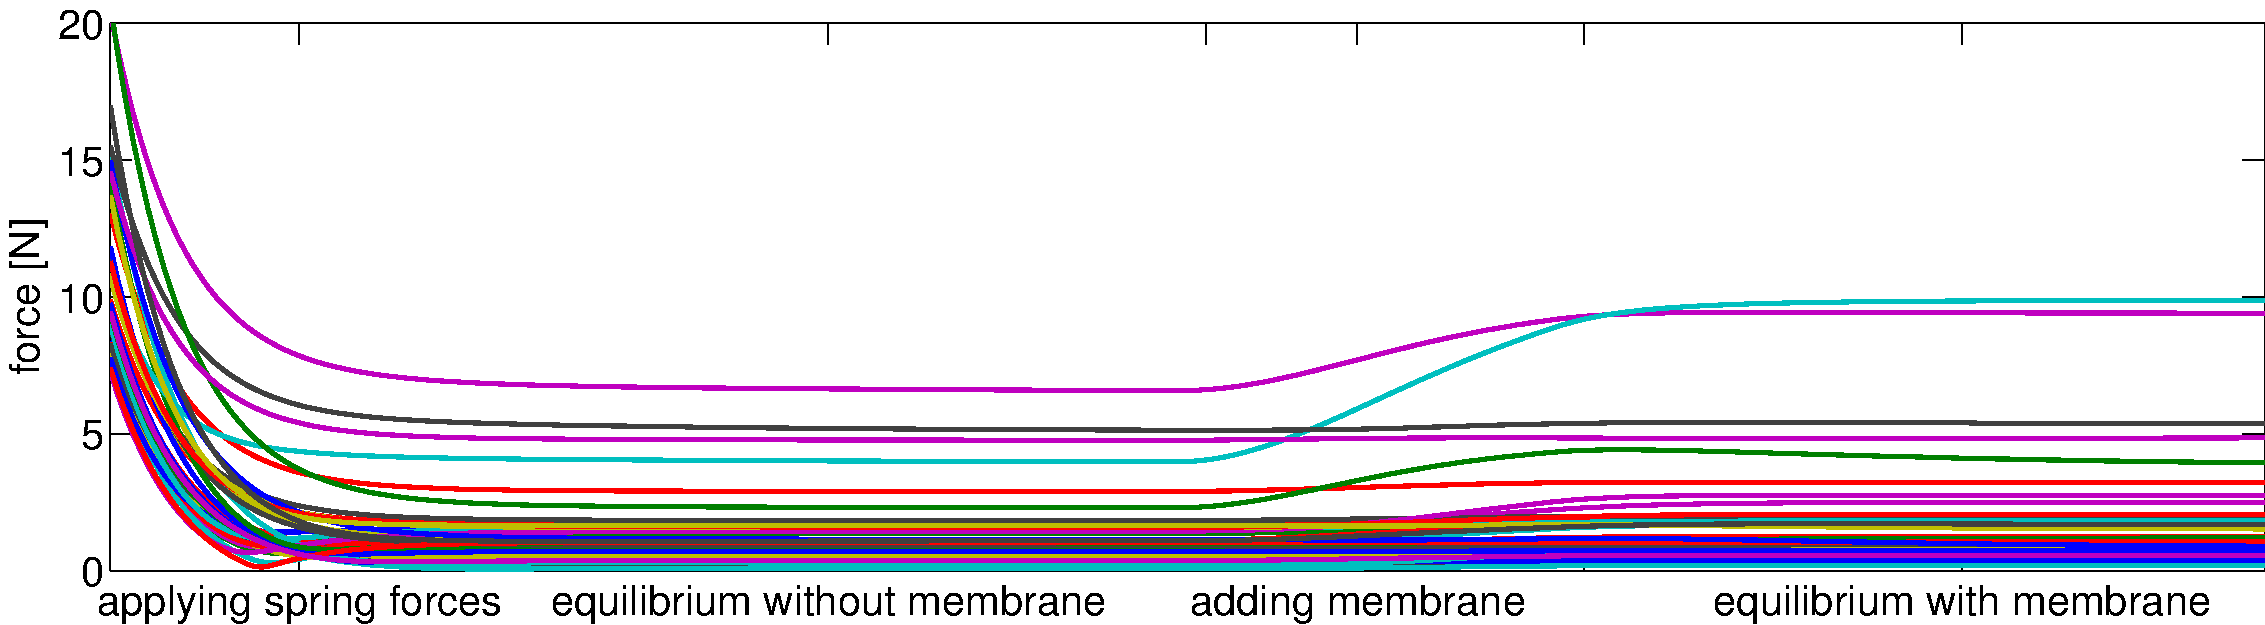
\includegraphics[width=.95\textwidth]{forceEvolution.pdf}
%  \caption{\label{f:forceEvol}Evolution of forces during the simulation, where the supine data is deformed
%towards the flank shape, and the stiffness of the capsule is increased from 0 to 8.22\,MPa after the initial equilibrium is achieved.}
%\end{figure}

\subsection{Global Deformations} %{{{

In the previous section we have shown that the composite model of parenchyma and 
capsule can be used to reproduce the \emph{local} behaviour of the tissue. In the following, 
we first present a real-time complete model of entire liver built from image data. 
Second, using this model we demonstrate the \emph{global} mechanical influence of the capsule when 
the model undergoes large deformations. 

The complete model was constructed using contrast-enhanced CT data acquired on a female pig 
being positioned first in supine and then flank position. 
The liver and hepatic vein were segmented for both datasets  using semi-automatic methods available in ITKSnap~\footnote{www.itksnap.org}.
Further, an unstructured mesh was obtained from the segmented maps using CGAL~\footnote{www.cgal.org}. 
The semi-automatic method presented in~\cite{Peterlik2012} was 
then applied to the segmented map of the hepatic vein, resulting in linked-beam model. 
Finally, the model of the Glisson's capsule was constructed using the elements described in 
section~\ref{ss:capsuleModel} over the surface triangles extracted from the tetrahedral mesh. 
The complete model composed of 4266 tetrahedra, 188 beams and 1284 triangles was then 
used in simulation where external force representing the gravity was applied to the model, 
resulting in large deformations mainly in the area of lobes. The refresh rate of 22\,FPS 
was achieved on a desktop computer with Intel i7 CPU running at 3.4\,GHz and 8\,GB of memory. 
The simulation with gravity was also used as a first demonstration of the global influence of the capsule. 
In Fig.~\ref{f:global}a, the models with capsule (red) and without (yellow) are depicted after being 
deformed due to the gravity, showing a significant difference between the two models.  

%XXX
%\begin{figure}[t]
%  \centering
%    \subfigure[]{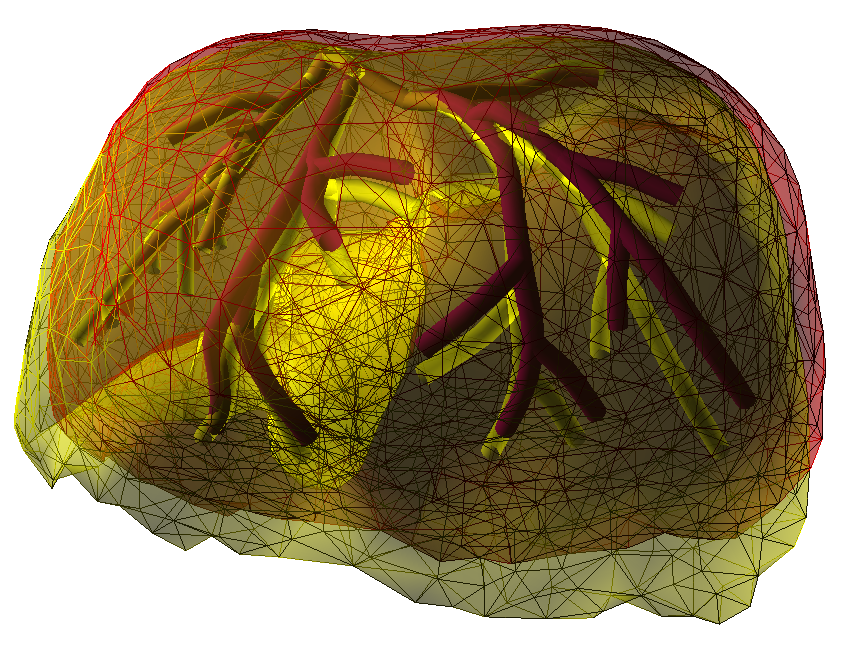
\includegraphics[width=.32\textwidth]{gravity2.png}}
%    \subfigure[]{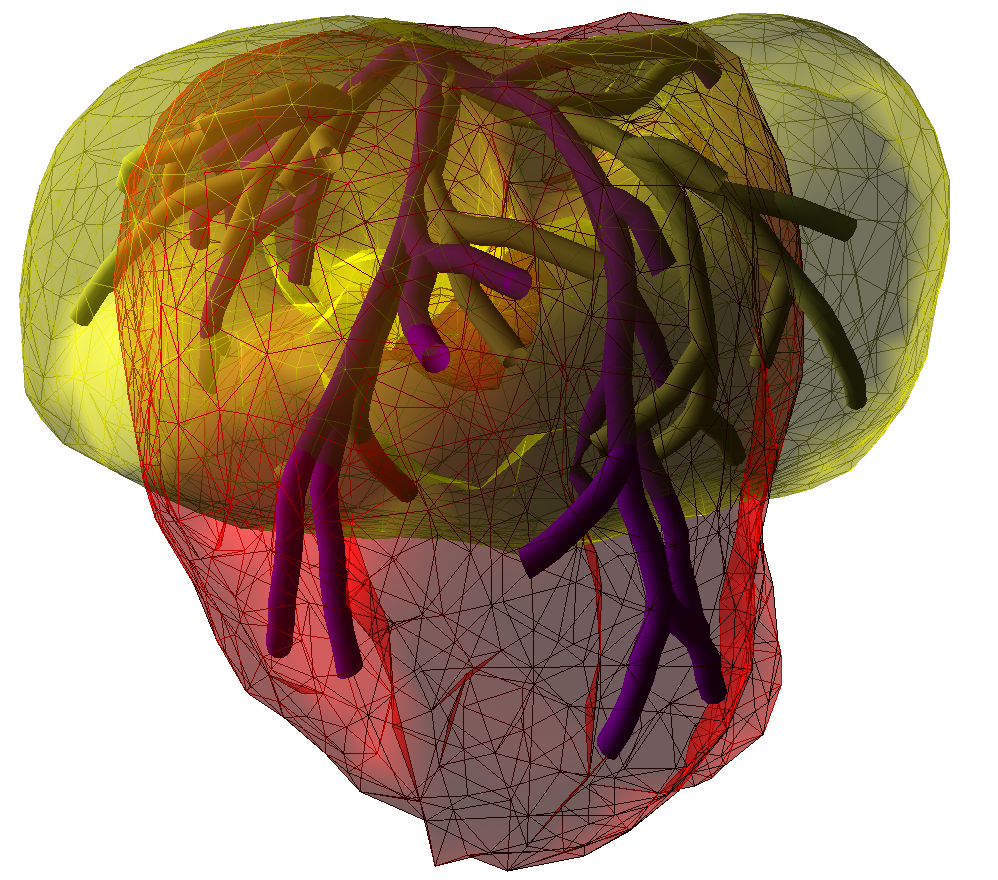
\includegraphics[width=.32\textwidth]{registered.png}}
%    \subfigure[]{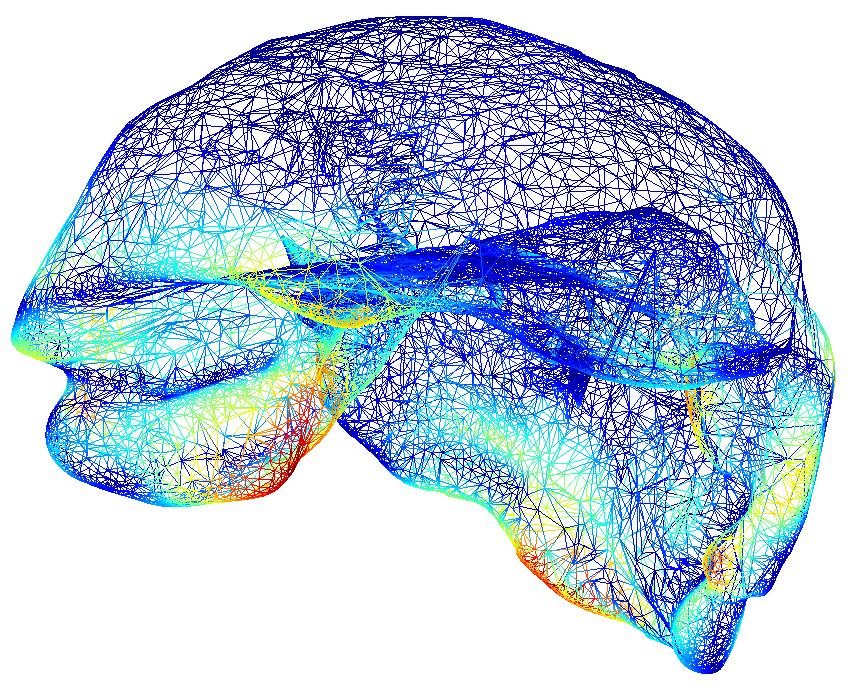
\includegraphics[width=.32\textwidth]{distanceMap.png}}
%    \caption{\label{f:global}%
%      (a) Liver under gravity with (red) and without (yellow) capsule;
%      (b) liver in supine (yellow) and flank (red) position;
%      (c) Hausdorff distance map between registered version with and without capsule.}
%\end{figure}

In order to demonstrate the influence of the capsule on a real deformation of the liver, we 
performed a following protocol employing the supine and flank models built from the CT data. 
First, we performed a rigid registration of the two organs \wrt the root point of the hepatic vein. 
As shown in Fig.~\ref{f:global}b, the liver undergoes very large deformation when the body 
is turned from the supine to the flank position, exceeding 6\,cm for some parts of the organ. 
In order to induce similar deformation, we extracted feature pairs from the vascular system of the liver:
we selected points such as bifurcations which can be identified easily in both supine and flank 
data resulting in a set of correspondences. In the next step, we used these correspondences as a non-homogeneous
boundary conditions (imposed via penalty term) in order to perform a deformable registration of the supine
model onto the flank data. During the registration, the response forces acting in the points with prescribed displacements
were calculated. It is important to emphasize that the goal of the simulation was not 
to perform an accurate registration of the flank and supine data, but the simulation was used 
as an example of a real deformation of the organ.

The simulation was performed with the model composed of parenchyma,  vessels and capsule, however, zero stiffness was 
set for the last component.
Once the static equilibrium was achieved, the effect of the capsule was gradually switched 
on, \ie the stiffness of the membrane was slowly increased from 0 to 8.22\,MPa. The evolution of the force response in the 
points with prescribed displacements is depicted in Fig.~\ref{f:forceEvol} showing the change in the response as the effect
of the capsule is included. At the same time, the shape of the deformed liver with capsule was compared 
to the model without the capsule. A Hausdorff distance map for those cases is depicted in Fig.~\ref{f:global}c: in the red areas, the 
maximal difference exceeding 1.25\,cm was measured. We believe that this result confirms that the Glisson's capsule 
plays an important role in the global mechanical behaviour of the liver.

%}}}

\subsection{More Experiments}

\TG{list of other experiments}

%}}}


\section{Conclusions} %{{{
In the paper, a complete model of the liver was presented taking into account 
three constituents of the organ, each being modelled with a different type 
of finite elements: tetrahedral corotational model used for the parenchyma, serially 
linked corotational beams based on Tymoshenko formulation employed to model the vascularization 
and finally CST elements used for the capsule. 
The model was first validated for local displacements: the aspiration test presented in~\cite{Hollenstein2006} 
was successfully reproduced, showing a good agreement between the simulation and experiments. 
Further, the model was used to demonstrate global influence of the capsule when the organ 
undergoes large deformations. 

In the future work, we plan to employ the proposed model for other organs where the capsule play an important role
(for example kidneys). We will also focus on better description of the mechanical interactions and couplings among the organs and tissues in the abdominal 
cavity via realistic modeling of boundary conditions using mechanical constraints and contacts.

%While the influence of the capsule on local deformations was previously
%studied in the literature, it's significance on the global scale
%deformations of the liver remained unexplored. We have performed a set of
%natural global deformations of the complete liver and shown that the
%capsule, despite its small thickness, plays a significant role also in
%global context.
%
%}}}

%% The Appendices part is started with the command \appendix;
%% appendix sections are then done as normal sections
%% \appendix

%% \section{}
%% \label{}

% ---  Bibliography  ---

\bibliographystyle{model1-num-names}
\bibliography{bibdata}

%% Authors are advised to submit their bibtex database files. They are
%% requested to list a bibtex style file in the manuscript if they do
%% not want to use model1-num-names.bst.

\end{document}
% spell: setl spell spelllang=en spellfile=spelldict.en.utf-8.add
% vim:set et sw=2 tw=75 fdm=marker fdl=3 fdc=4 isk+=_,-:
